% This is samplepaper.tex, a sample chapter demonstrating the
% LLNCS macro package for Springer Computer Science proceedings;
% Version 2.21 of 2022/01/12
%
\documentclass[runningheads]{llncs}
%
\usepackage[T1]{fontenc}
% T1 fonts will be used to generate the final print and online PDFs,
% so please use T1 fonts in your manuscript whenever possible.
% Other font encondings may result in incorrect characters.
%
\usepackage{graphicx}
% Used for displaying a sample figure. If possible, figure files should
% be included in EPS format.
%
% If you use the hyperref package, please uncomment the following two lines
% to display URLs in blue roman font according to Springer's eBook style:
%\usepackage{color}
%\renewcommand\UrlFont{\color{blue}\rmfamily}
%\urlstyle{rm}
%

\usepackage{algorithm}
\usepackage{algpseudocode}
\usepackage{amsmath}

\begin{document}
%
\title{Decision-making via evidence accumulation and metacognitive self-regulation}
%
%\titlerunning{Abbreviated paper title}
% If the paper title is too long for the running head, you can set
% an abbreviated paper title here
%
\author{Baptiste Pesquet \and Frédéric Alexandre}
%
\authorrunning{B. Pesquet and F. Alexandre.}
% First names are abbreviated in the running head.
% If there are more than two authors, 'et al.' is used.
%
\institute{INRIA, University of Bordeaux, CNRS, Bordeaux INP - France}
%
\maketitle              % typeset the header of the contribution
%
\begin{abstract}
Human cognition is distinguished not only by the ability to make decisions and learn from experience, but also by the capacity to reflect on and regulate these very processes — a faculty known as metacognition. Current AI systems largely lack this self-regulatory capacity. Inspired by models of sequential decision-making in humans and animals, we propose a modular architecture for a metacognitive artificial agent. Actions are selected via a novel decision-making module that accumulates evidence rather than applying a standard reinforcement learning policy. Confidence is derived from the accumulation results at decision time and used to dynamically adjust learning and decision hyperparameters, implementing metacognitive self-regulation. To evaluate this architecture, we introduce a collaborative object-sorting task in which a learning agent must coordinate with a deterministic partner. Preliminary results show that the metacognitive agent reaches competitive performance relative to a standard Q-Learning and a deeper Q-network agent. These findings suggest that integrating confidence-driven self-regulation into learning agents is a promising direction toward more adaptive and cognitively plausible artificial intelligence.

\keywords{Decision-making \and Reinforcement Learning \and Metacognition.}
\end{abstract}
%
%
%
\section{Motivation}

Decision-making and learning are two hallmarks of cognition, and mutually influential processes \cite{mileticNewModelDecision2021}. Both are key skills to adapt to one's environment and reach one's goals. Advances in artificial intelligence (AI), particularly in large language models \cite{radfordImprovingLanguageUnderstanding} and reinforcement learning (RL) systems \cite{suttonReinforcementLearningIntroduction2018}, have narrowed the gap between artificial and human aptitudes in these fields. Yet, human cognition remains characterized by several key traits: ability to generalize from few examples, adaptability to uncertainty and changes in the environment, capacity to define one's own goals and explain one's behavior, and ability to evaluate and control one's mental processes (\textit{metacognition}). Despite recent progress \cite{weiChainofThoughtPromptingElicits2023} \cite{botvinickReinforcementLearningFast2019}, current AI systems mostly excel at reactive, implicit decision-making and struggle to replicate the flexibility of human cognition.

Inspired by research in experimental psychology and cognitive modeling, we propose an architecture for an artificial agent augmented with metacognitive abilities. Its decision-making and learning capabilities are evaluated through an original object sorting task.

\section{Related work}

A decision is a deliberative process that results in the commitment to a categorical proposition \cite{goldNeuralBasisDecision2007}. Some cognitive models of decision-making envision a decision as an accumulation-to-threshold operation. These are known as \textit{sequential sampling models} or \textit{evidence accumulation models} (EAM) \cite{forstmannSequentialSamplingModels2016}. Another class of models combines reinforcement learning and evidence accumulation in order to explicit the mutual interactions between learning and decision-making \cite{mileticNewModelDecision2021}.

The framework of reinforcement learning, in which an agent learns to gradually refine its behavior to maximize a cumulative reward, draws on foundational ideas from behavioral psychology. Similarities at both the behavioral and computational levels have been reported with reactive decision-making in animals \cite{suriNeuralNetworkModel1999}. The addition of Deep Learning techniques has given birth to powerful new methods in the field \cite{mnihHumanlevelControlDeep2015}. Another line of research augments RL with episodic or working memory systems, extending its use to non-Markovian contexts \cite{zilliModelingRoleWorking2008}. Other approaches try to give agents the ability to choose actions at different time scales, paving the way for deliberative decision-making and goal-directed behavior \cite{stolleLearningOptionsReinforcement2002}, \cite{baconOptionCriticArchitecture2016}.

Metacognition, the capacity to reflect on and regulate one's own mental functions, is a defining trait of natural cognition \cite{flemingMetacognitionConfidenceReview}. Metacognition is generally divided into two subprocesses: \textit{monitoring} and \textit{control}. Monitoring refers to the evaluation of several latent quantities (errors, conflicts, uncertainties, etc) about other mental operations. Control refers to the exploitation of these signals for self-regulation, for example by inhibiting the default behavior to favor adaptation to a specific context. A key part of metacognitive monitoring consists of \textit{confidence judgments}, quantifying the degree of certainty associated with decisions. Some cognitive models of sequential decision-making derive confidence from the difference between accumulators for each alternative. A larger gap is associated with a higher degree of confidence, reflecting a more robust decision. Furthermore, this approach is biologically grounded \cite{kepecsNeuralCorrelatesComputation2008}. Other models use confidence as the switch mechanism between different behavior rules \cite{collinsReasoningLearningCreativity2012}. However, the evaluation and exploitation of confidence in metacognitive models of decision-making is still a poorly understood topic.

\section{Methodology}

\subsection{Proposed architecture}

Taking into account previous literature on confidence and human decision-making, we designed a model for an artificial agent using a cognitively plausible architecture for learning and decision-making. It has four tightly coupled modules (Figure \ref{fig:agent_architecture}):

\begin{itemize}
  \item The \textbf{Perception} module receives raw observations from the environment and encodes them into a vectorized state representation.
  \bigskip 
  \item The \textbf{Learning} module implements the RL framework. Receiving the state, it maintains a list of action value estimations (Q-values) for each action/state pair. These values are updated via Q-Learning (Equation \ref{eq:q_learning}), classically using the reward prediction error $\delta$ (Equation \ref{eq:rpe}).

\begin{equation}
\delta = R + \gamma \cdot \max_a Q(S',a) - Q(S,A)
\label{eq:rpe}
\end{equation}

\begin{equation}
Q(S,A) \leftarrow Q(S,A) + \alpha \cdot \delta
\label{eq:q_learning}
\end{equation}

  \bigskip 
  \item The \textbf{Decision-making} module represents the core novelty of our work. Rather than directly deriving a policy from the Q-values (e.g. $\epsilon$-greedy), it selects actions via  evidence accumulation \cite{mileticNewModelDecision2021}. At each environment time step, the module runs one accumulator per directional pairwise difference between Q-values, leading to a total of $n(n-1)$ accumulators for $n$ possible actions. Each pairwise accumulator $x_{i,j}$ collects evidence for action $a_i$ over action $a_j$ (Equation \ref{eq:ard_acc}). All accumulators race toward a common threshold $\theta$. The speed of evidence accumulation $v_{i,j}$, called the \textit{drift rate} of the accumulator, is defined as a weighted sum between the \textit{advantage} (difference) term that captures relative preference between $a_i$ and $a_j$, the \textit{sum} term that captures absolute magnitude, and a stimulus-independent urgency baseline (Equation \ref{eq:ard_drift_rate}). A decision is made for action $a_i$ once all its accumulators $x_{i,\cdot}$ have crossed $\theta$, implementing a "win-all" stopping rule \cite{vanravenzwaaijAccumulatingAdvantagesNew2020}. The confidence associated with the decision is computed as the normalised distance between winner's and runner-up's slowest accumulators at decision time (Figure \ref{fig:ard_dynamics}).

\begin{equation}
v_{i,j} = w_d\big(Q(S,a_i)-Q(S,a_j)\big) + w_s\big(Q(S,a_i)+Q(S,a_j)\big) + V_0
\label{eq:ard_drift_rate}
\end{equation}

\begin{equation}
\text{d}x_{i,j} = v_{i,j}\text{d}t + \text{noise}
\label{eq:ard_acc}
\end{equation}

  \bigskip 
  \item The \textbf{Metacognition} module exploits the confidence $c$ computed at decision time to dynamically adjust two \textit{hyperparameters} of the model: the decision threshold $\theta$ (Equation \ref{eq:meta_theta}) and the Q-value learning rate $\alpha$ (Equation \ref{eq:meta_alpha}). A low value of confidence compared to a desired level $c_{target}$ raises both $\theta$ (forcing more evidence for the next decisions) and $\alpha$ (updating beliefs more aggressively in presence of uncertainty). A high level of confidence triggers the opposite effects.

\begin{equation}
\theta \gets \theta - \eta_{\theta}(c - c_{target})
\label{eq:meta_theta}
\end{equation}

\begin{equation}
\alpha \gets \alpha - \eta_{\alpha}(c - c_{target})
\label{eq:meta_alpha}
\end{equation}

\end{itemize}

\begin{figure}
\centering
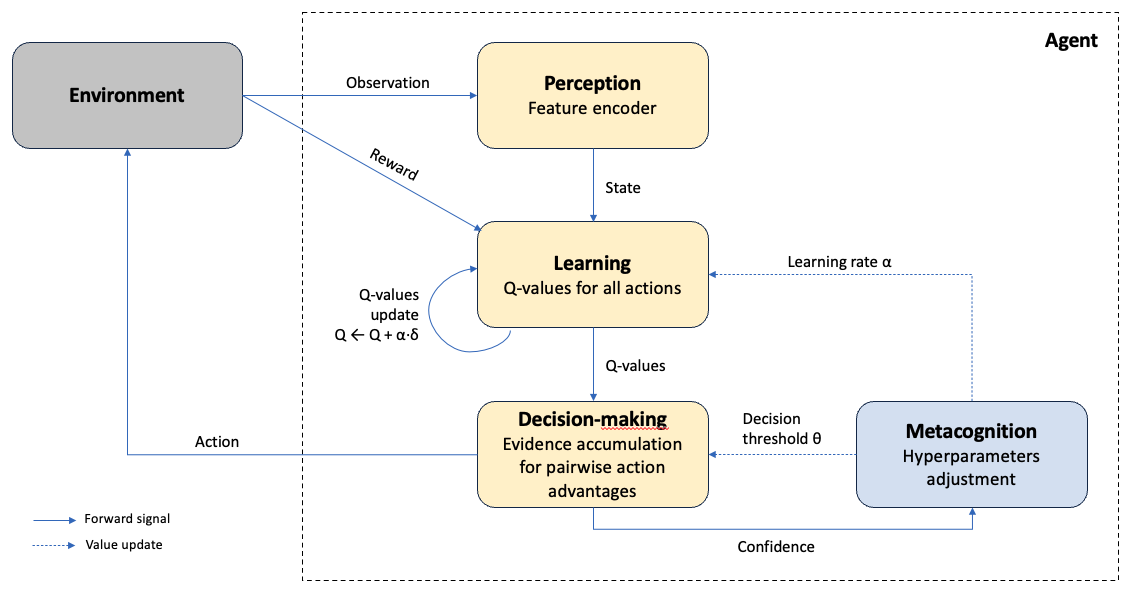
\includegraphics[width=0.95\textwidth]{img/agent_architecture.png}
\caption{The proposed architecture for a metacognitive agent interacting with its environment. The \textbf{Perception} module turns the received observation into a discrete state. The \textbf{Learning} module maintains Q-values for all known action/state pairs. These values are updated after a reward is received, using the reward prediction error $\delta$. They are used by the \textbf{Decision-making} module to drive evidence accumulation for all pairwise differences between Q-values. The first action for which all pairwise accumulators cross the decision threshold $\theta$ is selected. The difference between accumulators at decision time is used to compute confidence, subsequently used by the \textbf{Metacognition} module to adjust $\theta$ and the Q-values learning rate $\alpha$.} \label{fig:agent_architecture}
\end{figure}

\begin{figure}
\centering
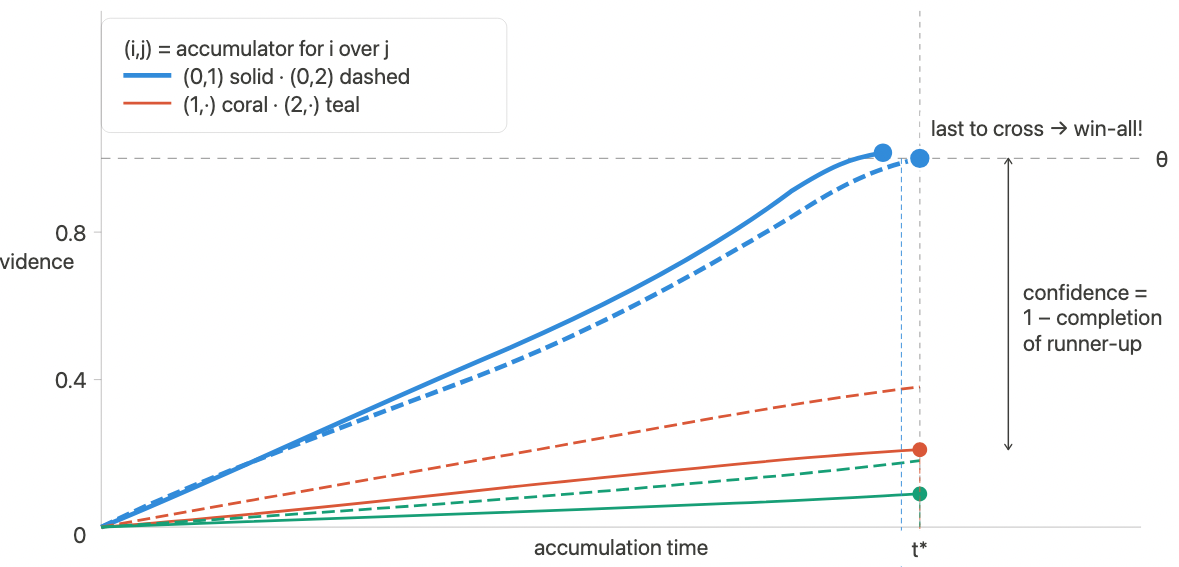
\includegraphics[width=0.95\textwidth]{img/ard_accumulation.png}
\caption{Illustration of the evidence accumulation dynamics for decision-making. Each of the three possible actions is associated with two accumulators representing the pairwise advantages over other actions. All accumulators are driven by their own drift rate (Equation \ref{eq:ard_drift_rate}). A decision is made once all accumulators for an action reach the threshold $\theta$. Confidence is computed at decision time as the normalized gap between best and second best actions' slowest accumulators. The horizontal axis represents the temporal unfolding of the decision. This accumulation process is fully encapsulated inside a single environment time step.} \label{fig:ard_dynamics}
\end{figure}

\subsection{Test environment}

In order to compare agent architectures, a dedicated task has been designed from the ground up. It is a simplified version of an experimental protocol established for a human-robot collaboration project: two agents represented as robotic arms must pick and place a series of objects moving in front of them (Figure \ref{fig:collabsort_task}). Rewards for picking an object are agent-specific and depend on object properties (shape and color). They may evolve between episodes, introducing volatility for agents. Collisions between arms are penalized through negative rewards. 

One of the agents is deterministic and selfish. It has access to all environment information, knows the initial object reward structure and uses hardcoded behavioral rules to pick objects. The other agent is used to compare different cognitive and metacognitive architectures. It has to learn how to maximize its cumulative reward while adapting to the other agent's behavior and to uncertainties in the environment.

The task is implemented in Python as a Gymnasium \cite{kwiatkowskiGymnasiumStandardInterface2024} environment. The scene is modelled as a gridworld-like 2D board of 10 by 10 squares. At each time step, all objects move by one square from right to left until they disappear from the board or are picked by a robotic arm. The environment state is provided to each agent as a dictionary containing:

\begin{itemize}
    \item The current $(x,y)$ coordinates of its arm gripper on the board.
    \item A boolean indicating if an object is currently picked by the gripper.
    \item The current $(x,y)$ coordinates of the other agent's arm gripper.
    \item The $(x,y)$ coordinates and properties (shape and color) of all object currently moving on the board.
\end{itemize}

At each time step, both agents select one action between four possibilities:

\begin{itemize}
    \item Moving the gripper up by one square, thus extending (for the agent at the bottom) or retracting (for the agent at the top) their arm.
    \item Moving the gripper down by one square, thus retracting (for the agent at the bottom) or extending (for the agent at the top) their arm.
    \item Picking an object, which must occupy the same square as the arm gripper for the action to be successful.
    \item Doing nothing.
\end{itemize}

Once an object is picked, the agent immediately gains the associated reward and its arm automatically retracts to its base in the subsequent time steps. Then, the object is placed alongside the robotic arm base and the agent can choose actions again.

The source code of the environment is available online \footnote{https://github.com/bpesquet/gym-collabsort}.

\begin{figure}
\centering
\fbox{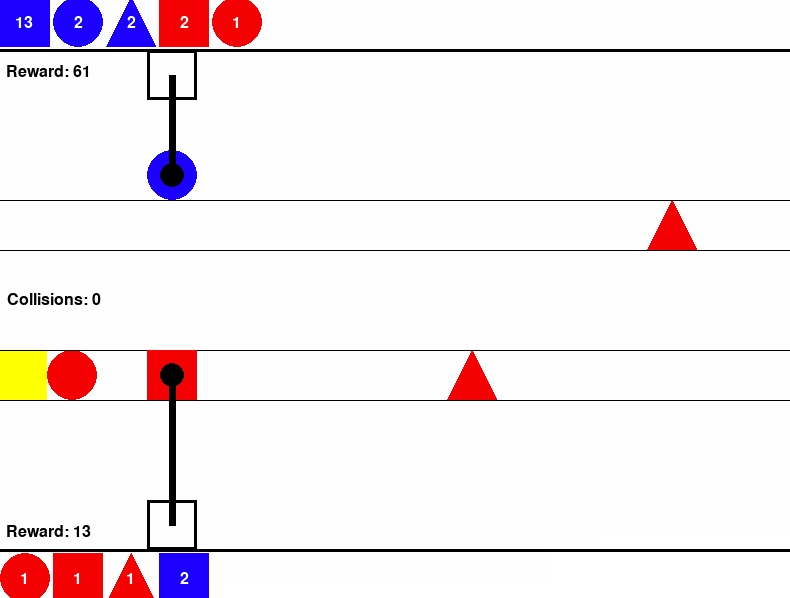
\includegraphics[width=0.75\textwidth]{img/collabsort_demo.jpg}}
\caption{The collaborative object sorting task used as test environment. Objects are moving from right to left on two horizontal treadmills. Each agent is represented by a vertically moving arm extending from a square base and terminated by a round gripper. Agents can only pick an object when it is at the same location as their arm gripper. The agent at the top is deterministic. The one at the bottom implements different cognitive and metacognitive architectures.} \label{fig:collabsort_task}
\end{figure}

\section{Preliminary results}

Three different architectures have been implemented so far for the cognitive agent:

\begin{itemize}
    \item An $\epsilon$-greedy policy based on tabular Q-Learning.
    \item An $\epsilon$-greedy policy based on a Q-network (two hidden layers of 100 artificial neurons each), using a target network and experience replay.
    \item A metacognitive policy combining evidence accumulation as described above and tabular Q-Learning.
\end{itemize}

All models were trained for 300 episodes of 1000 timesteps against the test environment. Rewards were fixed during training (no volatility). To account for the imperfect perceptual abilities of agents, only the objects located on the same column as the robotic arms and on the two preceding columns were considered as perceived and included into the state sent to the Learning module.

Preliminary results (Figure \ref{fig:res_ard_eps}, Figure \ref{fig:res_ard_dqn}) demonstrate the validity of our approach. The metacognitive agent is able to match the level of performance of an $\epsilon$-greedy policy while being faster in terms of learning. The Q-network agent obtains slightly better results, but it also learns slower than the metacognitive agent.

Ongoing works are carried out to consolidate these first results, add sources of uncertainties to the environment, study the impacts of $\theta$ and $\alpha$ adjustments separately, improve the metacognitive architecture and compare it to more reinforcement learning algorithms.

The source code of all experiments is available online \footnote{https://github.com/bpesquet/collabsort-agent}.

\begin{figure}
\centering
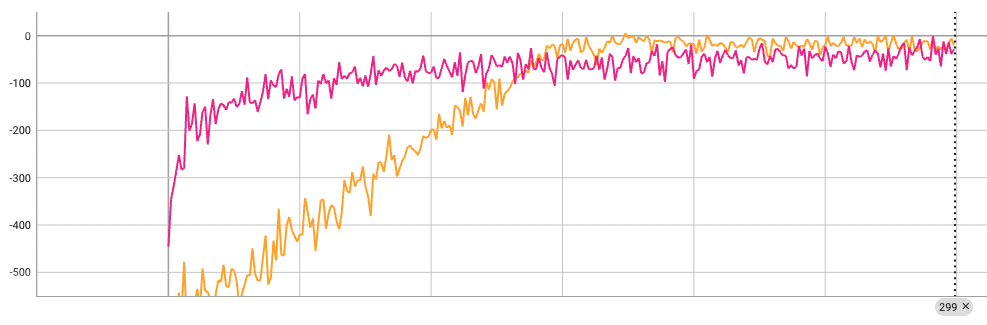
\includegraphics[width=0.8\textwidth]{img/results_ard_eps.png}
\caption{Cumulated rewards at the end of episodes for the metacognitive (magenta) and Q-Learning (orange) agents. The former learns faster while reaching similar results.} \label{fig:res_ard_eps}
\end{figure}

\begin{figure}
\centering
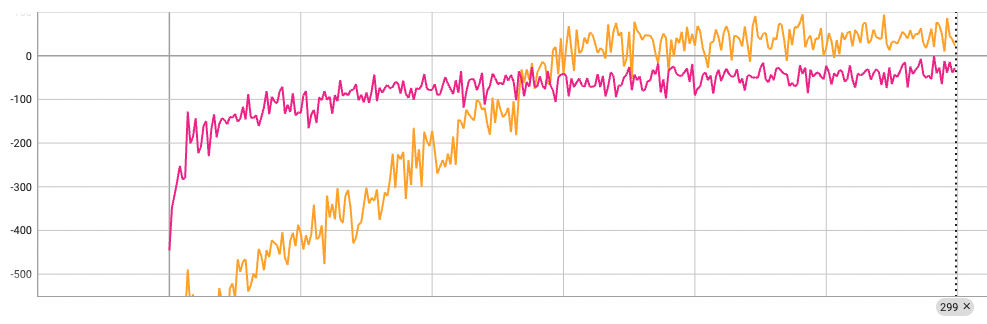
\includegraphics[width=0.8\textwidth]{img/results_ard_dqn.png}
\caption{Cumulated rewards at the end of episodes for the metacognitive (magenta) and Q-network (orange) agents. The latter obtains better results overall, but the former learns faster.} \label{fig:res_ard_dqn}
\end{figure}

\section{Conclusion and perspectives}

Building from research at the crossroads of artificial intelligence and cognitive computational neuroscience, we developed a metacognitive artificial agent capable of assessing its own confidence levels and dynamically adjusting its decision-making accordingly. A dedicated testbed inspired by a human-robot collaboration project has been created to assess the agent's abilities and compare them to more standard approaches.

Future work will focus on refining and expanding the cognitive architecture to address broader aspects of metacognition. A future objective would be to augment the metacognitive agent with the ability to learn behavior rules instead of merely action values. Another potentially fruitful avenue would be to handle collaborative aspects by tracking \textit{social uncertainty}: the level of confidence regarding partner predictability could be computed and used to adjust the agent's behavior. Ultimately, our efforts are oriented toward more autonomous and flexible artificial agents.
%
% ---- Bibliography ----
%
% BibTeX users should specify bibliography style 'splncs04'.
% References will then be sorted and formatted in the correct style.
%
\bibliographystyle{splncs04}
\bibliography{bibliography}

\end{document}
